% LaTeX source for ``Think Bayes: Bayesian Statistics Made Simple''
% Copyright 2012  Allen B. Downey.

% License: Creative Commons Attribution-NonCommercial 3.0 Unported License.
% http://creativecommons.org/licenses/by-nc/3.0/
%

\documentclass[12pt]{book}
\usepackage[width=5.5in,height=8.5in,
  hmarginratio=3:2,vmarginratio=1:1]{geometry}

% for some of these packages, you might have to install
% texlive-latex-extra (in Ubuntu)

\usepackage[T1]{fontenc}
\usepackage{textcomp}
\usepackage{mathpazo}
\usepackage{url}
\usepackage{fancyhdr}
\usepackage{graphicx}
\usepackage{subfig}
\usepackage{amsmath}
\usepackage{amsthm}
\usepackage{makeidx}
\usepackage{setspace}
\usepackage{hevea}                           
\usepackage{upquote}

\title{Think Bayes}
\author{Allen B. Downey}

\newcommand{\thetitle}{Think Bayes: Bayesian Statistics Made Simple}
\newcommand{\theversion}{0.2.0}

% these styles get translated in CSS for the HTML version
\newstyle{a:link}{color:black;}
\newstyle{p+p}{margin-top:1em;margin-bottom:1em}
\newstyle{img}{border:0px}

% change the arrows in the HTML version
\setlinkstext
  {\imgsrc[ALT="Previous"]{back.png}}
  {\imgsrc[ALT="Up"]{up.png}}
  {\imgsrc[ALT="Next"]{next.png}} 

\makeindex

\newif\ifplastex
\plastexfalse

\begin{document}

\frontmatter

\ifplastex

\else
\fi

\newcommand{\PMF}{\mathrm{PMF}}
\newcommand{\PDF}{\mathrm{PDF}}
\newcommand{\CDF}{\mathrm{CDF}}
\newcommand{\ICDF}{\mathrm{ICDF}}

\ifplastex
    \usepackage{localdef}
    \maketitle

\else

\input{latexonly}

\begin{latexonly}

\renewcommand{\blankpage}{\thispagestyle{empty} \quad \newpage}

% TITLE PAGES FOR LATEX VERSION

%-half title--------------------------------------------------
\thispagestyle{empty}

\begin{flushright}
\vspace*{2.0in}

\begin{spacing}{3}
{\huge Think Bayes}\\
{\Large Bayesian Statistics Made Simple}
\end{spacing}

\vspace{0.25in}

Version \theversion

\vfill

\end{flushright}

%--verso------------------------------------------------------

\blankpage
\blankpage

%--title page--------------------------------------------------
\pagebreak
\thispagestyle{empty}

\begin{flushright}
\vspace*{2.0in}

\begin{spacing}{3}
{\huge Think Bayes}\\
{\Large Bayesian Statistics Made Simple}
\end{spacing}

\vspace{0.25in}

Version \theversion

\vspace{1in}


{\Large
Allen B. Downey\\
}


\vspace{0.5in}

{\Large Green Tea Press}

{\small Needham, Massachusetts}

\vfill

\end{flushright}


%--copyright--------------------------------------------------
\pagebreak
\thispagestyle{empty}

Copyright \copyright ~2012 Allen B. Downey.


\vspace{0.2in}

\begin{flushleft}
Green Tea Press       \\
9 Washburn Ave \\
Needham MA 02492
\end{flushleft}

Permission is granted to copy, distribute, and/or modify this document
under the terms of the Creative Commons Attribution-NonCommercial 3.0 Unported
License, which is available at \url{http://creativecommons.org/licenses/by-nc/3.0/}.

\vspace{0.2in}

\end{latexonly}


% HTMLONLY

\begin{htmlonly}

% TITLE PAGE FOR HTML VERSION

{\Large \thetitle}

{\large Allen B. Downey}

Version \theversion

\vspace{0.25in}

Copyright 2012 Allen B. Downey

\vspace{0.25in}

Permission is granted to copy, distribute, and/or modify this document
under the terms of the Creative Commons Attribution-NonCommercial 3.0
Unported License, which is available at
\url{http://creativecommons.org/licenses/by-nc/3.0/}.

\setcounter{chapter}{-1}

\end{htmlonly}

\fi
% END OF THE PART WE SKIP FOR PLASTEX

\chapter{Preface}
\label{preface}

\section*{}

This version of the book is a rough draft.  I am making this draft
available for comments, but it comes with the warning that it is
probably full of errors.

If you find some of those errors, please let me know.  But it is
probably too early to bother with typos.

Allen B. Downey \\*
Needham MA \\*

Allen B. Downey is a Professor of Computer Science at 
the Franklin W. Olin College of Engineering.




%\section*{Acknowledgements}



\section*{Contributor List}

If you have a suggestion or correction, please send email to 
{\tt downey@allendowney.com}.  If I make a change based on your
feedback, I will add you to the contributor list
(unless you ask to be omitted).
\index{contributors}

If you include at least part of the sentence the
error appears in, that makes it easy for me to search.  Page and
section numbers are fine, too, but not quite as easy to work with.
Thanks!

\small

\begin{itemize}

\item First, I have to acknowledge David MacKay's excellent book,
  ``Information Theory, Inference, and Learning Algorithms'' which is
  where I first came to understand Bayesian methods.  With his
  permission (and with acknowledgement) I use several problems from
  his book as examples.

\item This book has also benefited from my interactions with Sanjoy
  Mahajan, especially in Fall 2012, when I audited his class on
  Bayesian Inference at Olin College.

% ENDCONTRIB

\end{itemize}

\normalsize

\clearemptydoublepage

% TABLE OF CONTENTS
\begin{latexonly}

\tableofcontents

\clearemptydoublepage

\end{latexonly}

% START THE BOOK
\mainmatter

\newcommand{\p}[1]{\ensuremath{\mathrm{p}(#1)}}
\newcommand{\T}[1]{\mbox{#1}}
\newcommand{\AND}{~\mathrm{and}~}
\newcommand{\NOT}{\mathrm{not}~}


\chapter{Bayes's Theorem}
\label{intro}

\section{Conditional probability}

The fundamental idea behind all Bayesian statistics is Bayes's Theorem,
which is surprisingly easy to derive, provided that you understand
conditional probability.  So we'll start with probability, then
conditional probabilty, then Bayes's Theorem, and on to Bayesian
statistics.

A probability is a number between 0 and 1 (including both) that
represents a degree of belief in a fact or prediction.  A probability
of 1 represents certainty that a fact is true, or that a prediction
will come true.  A probability of 0 represents equal certainty
that the fact is false.

Intermediate values represent degrees of certainty.  The value 0.5,
often represented as 50\%, means that a predicted outcome is
as likely to happen as not.  For example, the probability that a tossed
coin lands face up is very close to 50\%.

A conditional probability is a probability based on some background
information.  For example, I might be interested in the probability
that I will have a heart attack in the next year.  According to the
CDC, ``Every year about 785,000 Americans have a first coronary attack.
(\url{http://www.cdc.gov/heartdisease/facts.htm})''

The U.S. population is about 311 million, so the probability that a
randomly-chosen American will have a heart attack in the next year is
roughly 0.3\%.

But I am not a randomly-chosen American.  Epidemiologists have
identified many factors affect the risk of heart attacks; depending on
those factors, my risk might be higher or lower than average.

I am male, 45 years old, and I have
borderline high cholesterol.  Those factors increase my chances.
However, I have low blood pressure and I don't smoke, and
those factors decrease my chances.

Plugging everything into the online calculator at
\url{http://hp2010.nhlbihin.net/atpiii/calculator.asp}, I find that my
risk of a heart attack in the next year is about 0.2\%, slightly
less than the national average.
That value is a conditional probability, because it is based on
a number of factors that make up my ``condition.''

The usual notation for conditional probability is \p{A|B}, which
is the probability of $A$ given that $B$ is true.  In this
example, $A$ represents the prediction that I will have a heart
attack in the next year, and $B$ is the set of conditions I listed.


\section{Conjoint probability}

``Conjoint probability'' is a fancy way to say the probability that
two things are true.  I will write \p{A \AND B} to mean the
probability that $A$ and $B$ are both true.

If you learned about probability in the context of coin tosses and
dice, you might have learned the formula

\[ \p{A \AND B} = \p{A}~\p{B} \quad\mbox{WARNING: not always true}\]

For example, if I toss two coins, and $A$ means the first coin lands
face up, and $B$ means the second coin lands face up, then $\p{A} =
\p{B} = 0.5$, and sure enough, $\p{A \AND B} = \p{A}~\p{B} = 0.25$.

But this formula only works because in this case $A$ and $B$ are
independent; that is, the second event does not depend on the first.
If you tell me the first coin is heads, that does not change \p{B}.

Here is a different example where the events are not independent.
Suppose again that $A$ means the first coin lands face up, but let's
add $C$, which means that {\em both} coins land face up.  What is the
probability of both events, \p{A \AND C}?

These events are dependent because if we know whether or not $A$ is
true, that changes \p{C}.  Specifically, if $A$ is true then $\p{C}
= 0.5$; but if $A$ is false $\p{C} = 0$.

To be more correct, I should not say that \p{C} changes, but
rather that the conditional probabilities are different: $\p{C|A} = 0.5$
and $\p{C| \NOT A} = 0$.

In general, the probability of a conjunction is
%
\[ \p{A \AND C} = \p{A}~\p{C|A} \]
%
for any $A$ and $C$.  In this example, \p{A \AND C} = (0.5)(0.5) = 0.25.


\section{The girl named Florida problem}

Conditional probability is a simple enough idea, but it can be
tricky to apply.  One example is the ``girl named Florida problem,''
which I found in Leonard Mlodinow's book {\it The Drunkard's Walk}.

Before we get to Mlodinow's version of the problem, let's work
up to it with some simpler versions.

Suppose I tell you that I have two children (which is true) and
that the older one is a girl (also true).  If you don't know anything
else about my family, what is the probability that both of
my children are girls?

To keep things simple, you can assume that my children are not twins,
and that the probability that any child is a girl is 50\%.

The fact that the first child is a girl does not affect the probability
for the second girl, so
%
\[ \p{\T{two girls} | \T{older child is a girl}} = 1/2 \]
%
No problem so far.  Let's change it just a little.  Suppose that instead
of telling you that my older child is a girl, I mentioned something
about ``my daughter,'' which implies that at least one of my children
is a girl, but it doesn't tell you which one, and it doesn't tell
you anything about the other child.  In that case, what is the probability
that both children are girls?

You might be tempted to say that it doesn't make any difference and
the chance is still $1/2$.  But that's not right.

To see why, imagine 100 families with two children.
You would expect 25 of them to have two girls and 25 to have two
boys; another 25 would have an older daughter and a younger son,
and 25 would have an older son and a younger daughter.

If we select the families with at least one girl, that eliminates
25 families with two boys, leaving 75 families.  Of those, 25
have two girls, so:
%
\[ \p{\T{two girls} | \T{at least one child is a girl}} = 1/3 \]
%
And now we're ready for the girl named Florida.  Suppose I tell
you that I have two children, and one of them is a girl named
Florida.  What is the probability that both children are girls?

Most people have a strong intuition that the name of the child
is irrelevant, and therefore the answer is $1/3$.  But that's
not right (at least for the interpretation of the problem that
I think is most natural).

You can find a solution to this problem in my blog, {\it Probably
  Overthinking It} at
\url{http://allendowney.blogspot.com/2011/11/girl-named-florida-solutions.html}.

This problem is fun, in part because the result is
counterintuitive, but it comes with a warning.  Our
intuition for probability is sometimes very good, but sometimes
misleading.  So we will need to be careful.


\section{The Cookie Problem}

We'll get to Bayes's Theorem soon, but I want to motivate it with an
example called The Cookie Problem\footnote{Based on an example from
  \url{http://en.wikipedia.org/wiki/Bayes'_theorem} that is no longer
  there.}.  Suppose there are two bowls of cookies.  Bowl 1 contains
  30 vanilla cookies and 10 chocolate cookies.  Bowl 2 contains 20 of
  each.

Now suppose you choose one of the bowls at random and, without looking,
select a cookie at random.  The cookie is vanilla.  What is the probability
that it came from Bowl 1?

This is a conditional probability; we want \p{\T{Bowl 1} | \T{vanilla}},
but it is not obvious how to compute it.  On the other
hand, if we flip it around, it's very easy:
%
\p{\T{vanilla} | \T{Bowl 1}} = 3/4
%
Unfortunately, \p{A|B} is {\em not} the same as \p{B|A}.  But there
is a way to get from one to the other: Bayes's Theorem.


\section{Bayes's Theorem}

At this point we have everything we need to derive Bayes's Theorem.
We'll start with the observation that conjunction is commutative; that is
%
\[ \p{A \AND B} = \p{B \AND A} \]
%
for any events $A$ and $B$.

Next, we write the probability of a conjunction:
%
\[ \p{A \AND B} = \p{A}~\p{B|A} \]
%
And if we define $A$ and $B$ the other way
around, we can also write
%
\[ \p{B \AND A} = \p{B}~\p{A|B} \]
%
And that's all we need.  Pulling those pieces together, we get
%
\[ \p{B}~\p{A|B} = \p{A}~\p{B|A} \]
%
Which means there are two ways to compute the conjunction.
If you have \p{A}, you multiply by the conditional
probability \p{B|A}.  Or you can do it the other way around; if you
know \p{B}, you multiply by \p{A|B}.  Either way you should get
the same thing.

Finally we can divide through by \p{B}
%
\[ \p{A|B} = \frac{\p{A}~\p{B|A}}{\p{B}} \]
%
And that's Bayes's Theorem!  It doesn't look like much, but
it is a surprisingly powerful idea.

As an example, we can use it to solve the Cookie Problem.  I'll write
$B_1$ for the hypothesis that the cookie came from Bowl 1
and $V$ for the vanilla cookie.  Plugging in Bayes's Theorem
we get
%
\[ \p{B_1|V} = \frac{\p{B_1}~\p{V|B_1}}{\p{V}} \]
%
The term on the left is what we want: the probability of Bowl 1, given
that we chose a vanilla cookie.  The terms on the right are:

\begin{itemize}

\item \p{B_1}: This is the probability that we chose Bowl 1, unconditioned
by what kind of cookie we got.  Since the problem says we chose a
bowl at random, we can assume \p{B_1} = 1/2.

\item \p{V|B_1}: This is the probability of getting a vanilla cookie
from Bowl 1, which is 3/4.

\item \p{V}: This is the probability of drawing a vanilla cookie from
either bowl.  If we combine the two bowls, we get 50 vanilla and 30
chocolate cookies, so \p(V) = 5/8.

\end{itemize}

Putting it together, we have 
%
\[ \p{B_1|V} = \frac{(1/2)(3/4)}{5/8} \]
%
which reduces to 3/5.  So the vanilla cookie is a hint that
we probably chose Bowl 1, because vanilla cookies are more likely to
come from Bowl 1.

This example demonstrates one use of Bayes's Theorem: it provides
a process to get from \p{B|A} to \p{A|B}.  This strategy is useful
in cases, like the Cookie Problem, where it is easier to compute
the terms on the right side of Bayes's Theorem than the term on the
left.

\section{The diachronic interpretation}

There is another way to think of Bayes's Theorem: it gives us a
way to update the probability of a hypothesis, $H$, in light of
some body of data, $D$.

This way of thinking about Bayes's Theorem is called the
{\bf diachronic interpretation}.  ``Diachronic'' means that something
is happening over time; in this case there is an implicit notion
that the probability of the hypotheses changes, over time, as
we see new data.

Rewriting Bayes's Theorem with $H$ and $D$ yields:
%
\[ \p{H|D} = \frac{\p{H}~\p{D|H}}{\p{D}} \]
%
In this interpretation, each term has a name:

\begin{itemize}

\item \p{H} is the probability of the hypothesis before we see
the data, called the prior probability, or just {\bf prior}.

\item \p{H|D} is what we want to compute, the probability of
the hypothesis after we see the data, called the {\bf posterior}.
 
\item \p{D|H} is the probability of the data under the hypothesis,
called the {\bf likelihood}.

\item \p{D} is the probability of the data under any hypothesis,
called the {\bf normalizing constant}.

\end{itemize}

In some cases, we can compute the prior
based on background information.  For example, the Cookie
Problem specifies that we choose a bowl at random (and implies
that they have equal probability).

In other cases the prior
is subjective; that is, reasonable people might disagree,
either because they use different background information
or because they interpret the same information differently.

The likelihood is usually the easiest part to compute.  In the
Cookie Problem, if we know which bowl the cookie came from,
we can get the probability of getting a vanilla cookie by counting.

The normalizing constant can be tricky.  It is supposed to be the
probability of seeing the data under any hypothesis at all, but in the
most general case it is hard to see what that means.

Most often we simplify things by specifying a set of hypotheses
that are

\begin{description}

\item[Mutually exclusive:] which means that only one hypothesis in
the set can be true, and

\item[Collectively exhaustive:] which means that there are no other
possibilities; one of the hypotheses has to be true.

\end{description}

I use the word {\bf suite} for a set of hypotheses that has these
properties.

In the Cookie Problem, there are only two hypotheses---the cookie
came from Bowl 1 or Bowl 2---and they are mutually exclusive and
collectively exhaustive.

In that case we can compute \p{D} using the law of total probability,
which says that if there are two exclusive ways that something
might happen, you can add up the probabilities like this:
%
\[ \p{D} = \p{B_1}~\p{D|B_1} + \p{B_2}~\p{D|B_2} \]
%
Plugging in the values from the Cookie Problem, we have
%
\[ \p{D} = (1/2)~(3/4) + (1/2)~(1/2) = 5/8 \]
%
which is what we computed earlier by mentally combining the two
bowls.


\newcommand{\MM}{M\&M}

\section{The \MM~Problem}

\MM's are small candy-coated chocolates that come in a variety of
colors.  Mars, Inc., which makes \MM's, changes the mixture of
colors from time to time.

In 1995, they introduced blue \MM's.  Before then, the color mix in
a bag of plain M\&Ms was (30\% Brown, 20\% Yellow, 20\% Red, 10\%
Green, 10\% Orange, 10\% Tan).  Afterward it was (24\% Blue , 20\%
Green, 16\% Orange, 14\% Yellow, 13\% Red, 13\% Brown).

%\index{M\&M}

A friend of mine has two bags of \MM's, and he tells me
that one is from 1994 and one from 1996.  He won't tell me which is
which, but he gives me one \MM~from each bag.  One is yellow and
one is green.  What is the probability that the yellow one came
from the 1994 bag?

This problem is similar to the Cookie Problem, with the twist that I
draw one sample from each bowl/bag.  This problem also gives me a
chance to demonstrate the table method, which is useful for solving
problems like this on paper.  In the next chapter we will
solve them computationally.

The first step is to enumerate the hypotheses.  In this case there
are only two:

\begin{itemize}

\item A: the yellow \MM~is from 1994, which implies that green is
from 1996.

\item B: the yellow \MM~is from 1996 and green from 1996.

\end{itemize}

Now we construct a table with a row for each hypothesis and a
column for each term in Bayes's Theorem:

\begin{tabular}{|c|c|c|c|c|}
\hline
   & \p{H} & \p{D|H} & \p{H}~\p{D|H}  & \p{H|D}  \\
\hline
A  &  1/2  &  (20)(20)  &  200  &  20/27 \\
B  &  1/2  &  (10)(14)  &   70  &  7/27 \\
\hline
\end{tabular}

The first column has the priors.
Since there is one bag from 1994 and one from 1996,
it is reasonable to choose $\p{A} = \p{B} = 1/2$.

The second column has the likelihoods, which follow from the
information in the problem.  If $A$ is true, the yellow \MM~came from
1994 with probability 20\%, and the green came from 1996 with
probability 20\%.  Because the selections are
independent, we get the conjoint probability by multiplying.

The third column is just the product of the previous two.
The sum of this column, 270, is the normalizing constant.
To get the last column, which contains the posteriors, we divide
the third column by the normalizing constant.

That's it.  Simple, right?

Well, you might be bothered by one detail.  I wrote \p{D|H}
in terms of percentages, not probabilities, which means it
is off by a factor of 10,000.  But that
cancels out when we divide through by the normalizing factor, so
it doesn't affect the result.

When the set of hypotheses is mutually exclusive and collectively
exhaustive, you can multiply the probabilities by any factor,
if it is convenient, as long as you apply the same factor to the entire
column.


\section{The Monty Hall problem}

The Monty Hall problem might be the most contentious question in
the history of probability.  The scenario is simple, but the correct
answer is so counter-intuitive that many people just can't accept
it, and many smart people have embarrassed themselves not just by
getting it wrong but by arguing the wrong side, aggressively,
in public.

Monty Hall was the original host of the game show {\em Let's Make a
Deal}.  The Monty Hall problem is based on one of the regular
games on the show.  If you are on the show, here's what happens:

\begin{itemize}

\item Monty shows you three closed doors and tells you that there is a
  prize behind each door: one prize is a car, the other two are less
  valuable prizes like peanut butter and fake finger nails.  The
  prizes are arranged at random.

\item The object of the game is to guess which door has the car.  If
  you guess right, you get to keep the car.

\item So you pick a door, which we will call Door A.  We'll call the
  other doors B and C.

\item Before opening the door you chose, Monty increases the
  suspense by opening either Door B or C, whichever does not
  have the car.  (If the car is actually behind Door A, Monty can
  safely open B or C, so he chooses one at random).

\item Then Monty offers you the option to stick with your original
  choice or switch to the one remaining unopened door.

\end{itemize}

The question is, should you ``stick'' or ``switch'' or does it
make no difference?
\index{stick}
\index{switch}
\index{intuition}

Most people have the strong intuition that it makes no difference.
There are two doors left, they reason, so the chance that the car
is behind Door A is 50\%.

But that is wrong.  In fact, the chance of winning if you stick
with Door A is only 1/3; if you switch, your chances are 2/3.

By applying Bayes's Theorem, we can break this problem into simple
pieces, and maybe convince ourselves that the correct answer is,
in fact, correct.

To start, we should make a careful statement of the data.  In
this case $D$ consists of two parts: Monty chooses Door B,
and there is no car there.

Next we define three hypotheses: $A$, $B$ and $C$ represent the
hypothesis that the car is behind Door A, Door B or Door C.
Again, let's apply the table method:

\begin{tabular}{|c|c|c|c|c|}
\hline
   & \p{H} & \p{D|H} & \p{H}~\p{D|H}  & \p{H|D}  \\
\hline
A  &  1/3  &  1/2  &  1/6  &  1/3 \\
B  &  1/3  &  0  &   0  &  0 \\
C  &  1/3  &  1  &   1/3  &  2/3 \\
\hline
\end{tabular}

Filling in the priors is easy because we are told that the prizes
are arranged at random, which implies that the car is equally
likely to be behind any door.

Figuring out the likelihoods takes some thought, but with reasonable
care we can be confident that we have it right:

\begin{itemize}

\item If the car is actually behind A, Monty could safely open Doors
B or C.  So the probability that he chooses B is 1/2.  Since he
knows where the car is, the probability that there is no car there
is 1.

\item If the car is actually behind B, Monty does not open B, so the
probability of the data we saw is 0.

\item Finally, if the car is behind Door C, Monty opens B with probability
1 and finds no car there with probability 1.

\end{itemize}

Now the hard part is over; the rest is just arithmetic.  The
sum of the third column is 1/2.  Dividing through yields
$\p{A|D} = 1/3$ and $\p{C|D} = 2/3$.  So you are better off switching.

There are many variations of the Monty Hall problem.  One of the
strengths of the Bayesian approach is that it generalizes to handle
these variations.

For example, suppose that Monty always chooses B if he can, and
only chooses C if he has to (because the car is behind B).  In
that case the revised table is:

\begin{tabular}{|c|c|c|c|c|}
\hline
   & \p{H} & \p{D|H} & \p{H}~\p{D|H}  & \p{H|D}  \\
\hline
A  &  1/3  &  1  &  1/3  &  1/2 \\
B  &  1/3  &  0  &   0   &  0 \\
C  &  1/3  &  1  &   1/3  &  1/2 \\
\hline
\end{tabular}

The only change is \p{D|A}.  If the car is behind $A$, Monty can
chose to open B or C.  But in this variation he always chooses
B, so $\p{D|A} = 1$.

As a result, the likelihoods are the same for $A$ and $C$, and the
posteriors are the same: $\p{A|D} = \p{C|D} = 1/2$.  In this case, the
fact that Monty chose B reveals no information about the location of
the car, so it doesn't matter whether the contestant sticks or
switches.

On the other hand, if he had opened $C$, we would know $\p{B|D} = 1$.


\chapter{Computational statistics}

\section{Distributions}

In statistics a {\bf distribution} is a set of values and their
corresponding probabilities.

For example, if you roll a six-sided die, the set of possible
values is the numbers 1 to 6, and the probability associated
with each value is 1/6.

As another example, you might be interested in how many times each
word appears in common English usage.  You could build a distribution
that includes each word and how many time it appears.

In Python, you could represent a distribution with a dictionary that
maps from each value to its probability.  As an alternative, I have
written a class called {\tt Pmf} that represents a distribution.  PMF
stands for ``probability mass function'' which is the more specific
mathematical term for what I am calling a distribution.

{\tt Pmf} is defined in a Python module I wrote to accompany this
book, called {\tt thinkbayes.py}.  You can download it from
\url{http://thinkbayes.com/thinkbayes.py}.  To use {\tt Pmf} you
can import it like this:

\begin{verbatim}
from thinkbayes import Pmf
\end{verbatim}

The following code builds a Pmf to represent the distribution
of outcomes for a six-sided die:

\begin{verbatim}
pmf = Pmf()
for x in [1,2,3,4,5,6]:
    pmf.Set(x, 1/6.0)
\end{verbatim}

\verb"Pmf" creates an empty Pmf object with no values.  The
\verb"Set" method sets the probability associated with each
value to $1/6$.

Here's another example that counts the number of times each word
appears in a sequence:

\begin{verbatim}
pmf = Pmf()
for word in word_list:
    pmf.Incr(word, 1)
\end{verbatim}

\verb"Incr" increases the ``probability'' associated with each
word by 1.  If a word is not already in the Pmf, it is added.

I put ``probability'' in quotes because in this example, the
probabilities are not normalized; that is, they do not add up to 1.
So they are not true probabilities.

But in this example the word counts are proportional to the probabilities.
So after we count all the words, we can compute probabilities by
dividing through by the total number of words.  {\tt Pmf} provides
a method, \verb"Normalize", that does exactly that:

\begin{verbatim}
pmf.Normalize()
\end{verbatim}

Once you have made a Pmf object, you can ask for the probability
associated with any value:

\begin{verbatim}
print pmf.Prob('the')
\end{verbatim}

And that would print the frequency of the word ``the'' as a fraction
of the words in the list.

Pmf uses a Python dictionary to store the values and their
probabilities, so the values in the Pmf can be any hashable type.
The probabilities can be any numerical type, but they are usually
floating point numbers (type \verb"float").


\section{The Cookie Problem}

In the context of Bayes's Theorem, it is natural to use a Pmf
to map from each hypothesis to its probability.  In the Cookie
Problem, the hypotheses are $B_1$ and $B_2$.  In Python, I will
represent them with strings:

\begin{verbatim}
pmf = Pmf()
pmf.Set('Bowl 1', 0.5)
pmf.Set('Bowl 2', 0.5)
\end{verbatim}

This distribution, which contains the priors for each hypothesis,
is called (wait for it) the {\bf prior distribution}.

To update the distribution based on new data (the vanilla cookie),
we multiply each prior by the corresponding likelihood.  The likelihood
of drawing a vanilla cookie from Bowl 1 is 3/4.  The likelihood
for Bowl 2 is 1/2.

\begin{verbatim}
pmf.Mult('Bowl 1', 0.75)
pmf.Mult('Bowl 2', 0.5)
\end{verbatim}

\verb"Mult" does what you would expect.  It gets the probability
for the given value and multiplies by the given factor.

After this update, the distribution is no longer normalized, but
because these hypotheses are mutually exclusion and collectively
exhaustive, we can {\bf renormalize}:

\begin{verbatim}
pmf.Normalize()
\end{verbatim}

The result is a distribution that contains the posterior probability
for each hypothesis, which is called (wait now) the
{\bf posterior distribution}.

Finally, we can get the posterior for Bowl 1.

\begin{verbatim}
print pmf.Prob('Bowl 1')
\end{verbatim}

And the answer is 0.6.  You can download this example
from \url{http://thinkbayes.com/cookie.py}.


\section{The Bayesian framework}

Before we go on to other problems, I want to rewrite the code
from the previous section to make it more general.  First I'll
define a class to encapsulate the code related to this problem:

\begin{verbatim}
class Cookie(Pmf):
    def __init__(self, hypos):
        Pmf.__init__(self)
        for hypo in hypos:
            self.Set(hypo, 1)
        self.Normalize()
\end{verbatim}

A Cookie object is a Pmf that maps from hypotheses to their
probabilities.  The \verb"__init__" method gives each hypothesis
the same probability.  As in the previous section, there are
two hypotheses:

\begin{verbatim}
    hypos = ['Bowl 1', 'Bowl 2']
    pmf = Cookie(hypos)
\end{verbatim}

\verb"Cookie" provides an \verb"Update" method that takes
data as a parameter and updates the probabilities.

\begin{verbatim}
    def Update(self, data):
        for hypo in self.Values():
            like = self.Likelihood(hypo, data)
            self.Mult(hypo, like)
        self.Normalize()
\end{verbatim}

\verb"Update" loops through each hypothesis in the suite
and multiplies its probability by the likelihood of the
data under the hypothesis, which is computed by \verb"Likelihood":

\begin{verbatim}
    mixes = {
        'Bowl 1':dict(vanilla=0.75, chocolate=0.25),
        'Bowl 2':dict(vanilla=0.5, chocolate=0.5),
        }

    def Likelihood(self, hypo, data):
        mix = self.mixes[hypo]
        like = mix[data]
        return like
\end{verbatim}

\verb"Likelihood" uses \verb"mixes", which is a dictionary
that maps from the name of a bowl to the mix of cookies in
the bowl.

Here's what the update looks like:

\begin{verbatim}
    pmf.Update('vanilla')
\end{verbatim}

And then we can print the posterior probability of each hypothesis:

\begin{verbatim}
    for hypo, prob in pmf.Items():
        print hypo, prob
\end{verbatim}

The result is

\begin{verbatim}
Bowl 1 0.6
Bowl 2 0.4
\end{verbatim}

which is the same as what we got before.  This code is more complicated
than what we saw in the previous section.  One advantage is that it
generalizes easily to the case where we draw more than one cookie:

\begin{verbatim}
    dataset = ['vanilla', 'chocolate', 'vanilla']
    for data in dataset:
        pmf.Update(data)
\end{verbatim}

The other advantage is that it provides a framework for solving many
similar problems.  In the next section we'll solve the Monty Hall
problem computationally and then see what parts of the framework are
the same.

The code in this section is available from
\url{http://thinkbayes.com/cookie2.py}.


\section{The Monty Hall problem}

To solve the Monty Hall problem, I'll define a new class:

\begin{verbatim}
class Monty(Pmf):
    def __init__(self, hypos):
        Pmf.__init__(self)
        for hypo in hypos:
            self.Set(hypo, 1)
        self.Normalize()

    def Update(self, data):
        for hypo in self.Values():
            like = self.Likelihood(hypo, data)
            self.Mult(hypo, like)
        self.Normalize()
\end{verbatim}

So far \verb"Monty" and \verb"Cookie" are exactly the same.
And the code that creates the Pmf is the same, too, except for
the names of the hypotheses.

\begin{verbatim}
    hypos = 'ABC'
    pmf = Monty(hypos)
\end{verbatim}

Calling \verb"Update" is pretty much the same:

\begin{verbatim}
    data = 'B'
    pmf.Update(data)
\end{verbatim}

And the implementation of \verb"Update" is exactly the same:

\begin{verbatim}
    def Update(self, data):
        for hypo in self.Values():
            like = self.Likelihood(hypo, data)
            self.Mult(hypo, like)
        self.Normalize()
\end{verbatim}

The only part that requires some work is \verb"Likelihood".

\begin{verbatim}
    def Likelihood(self, hypo, data):
        if hypo == data:
            return 0
        elif hypo == 'A':
            return 0.5
        else:
            return 1
\end{verbatim}

Finally, printing the results is the same:

\begin{verbatim}
    for hypo, prob in pmf.Items():
        print hypo, prob
\end{verbatim}

And the answer is

\begin{verbatim}
A 0.333333333333
B 0.0
C 0.666666666667
\end{verbatim}

In this example, writing \verb"Likelihood" is a little complicated,
but the framework of the Bayesian update is simple.  The code in
this section is available from \url{http://thinkbayes.com/monty.py}.


\section{Encapsulating the framework}

Now that we see what elements of the framework are the same, we
can encapsulate them in an object: a \verb"Suite" is a \verb"Pmf"
that provides \verb"__init__", \verb"Update" and \verb"Print".

\begin{verbatim}
class Suite(Pmf):
    """Represents a suite of hypotheses and their probabilities."""

    def __init__(self, hypos):
        """Initializes the distribution."""

    def Update(self, data):
        """Updates each hypothesis based on the data."""

    def Print(self):
        """Prints the hypotheses and their probabilities."""
\end{verbatim}

The implementation of \verb"Suite" is in \verb"thinkbayes.py".  To use
\verb"Suite", you should write a class that inherits from it and
provides \verb"Likelihood".  For example, here is the solution to the
Monty Hall problem rewritten to use \verb"Suite":

\begin{verbatim}
from thinkbayes import Suite

class Monty(Suite):

    def Likelihood(self, hypo, data):
        if hypo == data:
            return 0
        elif hypo == 'A':
            return 0.5
        else:
            return 1
\end{verbatim}

And here's the code that uses this class:

\begin{verbatim}
    suite = Monty('ABC')
    suite.Update('B')
    suite.Print()
\end{verbatim}

You can download this example at
\url{http://thinkbayes.com/monty2.py}.  If you are familiar with
design patterns, you might recognize this as an example of the
Template method pattern: the parent class, \verb"Suite", defines an
algorithm framework; the child class, \verb"Monty" provides the
missing elements of the algorithm, in this case the \verb"Likelihood"
function.  You can read about this pattern at
\url{http://en.wikipedia.org/wiki/Template_method_pattern}.


\section{The \MM~problem}

We can use the \verb"Suite" framework to solve the \MM~problem.
Writing the \verb"Likelihood" function is tricky, but everything
else is straightforward.

First I need to encode the color mixes from before and
after 1995.

\begin{verbatim}
    mix94 = dict(brown=30,
                 yellow=20,
                 red=20,
                 green=10,
                 orange=10,
                 tan=10)

    mix96 = dict(blue=24,
                 green=20,
                 orange=16,
                 yellow=14,
                 red=13,
                 brown=13)
\end{verbatim}

Then I have to encode the hypotheses:

\begin{verbatim}
    hypoA = dict(bag1=mix94, bag2=mix96)
    hypoB = dict(bag1=mix96, bag2=mix94)
\end{verbatim}

\verb"hypoA" represents the hypothesis that Bag 1 is from
1994 and Bag 2 from 1996.  \verb"hypoB" is the other way
around.

Next I map from the name of the hypothesis to the representation:

\begin{verbatim}
    hypotheses = dict(A=hypoA, B=hypoA)
\end{verbatim}

And finally I can write \verb"Likelihood".  In this case
the hypothesis, \verb"hypo" is a string, \verb"A" or \verb"B".
The data is a tuple that specifies a bag, \verb"bag1" or \verb"bag2",
and a color.

\begin{verbatim}
    def Likelihood(self, hypo, data):
        bag, color = data
        mix = self.hypotheses[hypo][bag]
        like = mix[color]
        return like
\end{verbatim}

Here's the code that creates the suite and updates it:

\begin{verbatim}
    suite = M_and_M('AB')

    suite.Update(('bag1', 'yellow'))
    suite.Update(('bag2', 'green'))

    suite.Print()
\end{verbatim}

And here's the result:

\begin{verbatim}
A 0.740740740741
B 0.259259259259
\end{verbatim}

The posterior probability of A is approximately $20/27$, which
is what we got before.

The code in this section is available from
\url{http://thinkbayes.com/m_and_m.py}.


\chapter{Tanks and Trains}

\section{Which die was it?}

This problem is based on an example I saw in Sanjoy Mahajan's class
on Bayesian inference.

Suppose I have a box of dice that contains a 4-sided die, a 6-sided
die, an 8-sided die, a 12-sided die and a 20-sided die.  If you
have ever played Dungeons\&Dragons, you know what I am talking about.

Suppose I select a die from the box at random, roll it, and get a 6.
What is the probability that I rolled each die?

Let me suggest a three-step strategy for approaching a problem like this.

\begin{enumerate}

\item Choose a representation for the hypotheses.

\item Choose a representation for the data.

\item Write the likelihood function.

\end{enumerate}

In previous examples I used strings to represent hypotheses and
data, but for the die problem I'll use numbers.  Specifically,
I'll use the integers 4, 6, 8, 12, and 20 to represent hypotheses:

\begin{verbatim}
    suite = Dice([4, 6, 8, 12, 20])
\end{verbatim}

And integers from 1 to 20 for the data:

\begin{verbatim}
    suite.Update(6)
\end{verbatim}

I chose these representations because they make it easy to
write the likelihood function:

\begin{verbatim}
class Dice(Suite):
    def Likelihood(self, hypo, data):
        if hypo < data:
            return 0
        else:
            return 1.0/hypo
\end{verbatim}

Here's how \verb"Likelihood" works.  If \verb"hypo < data", that
means the roll is greater than the number of sides on the die.
That can't happen, so the likelihood is 0.

Otherwise the question is, ``Given that there are {\tt hypo}
sides, what is the chance of rolling {\tt data}?''  The
answer is \verb"1/hypo", regardless of {\tt data}.

You can download this example from \url{http://thinkbayes.com/dice.py}.
And here is the result:

\begin{verbatim}
4 0.0
6 0.392156862745
8 0.294117647059
12 0.196078431373
20 0.117647058824
\end{verbatim}

After we roll a 6, the probability for the 4-sided die is 0.  The
most likely alternative is the 6-sided die, but there is still
almost a 12\% chance for the 20-sided die.

What if we roll a few more times and get 6, 8, 7, 7, 5, and 4?

\begin{verbatim}
    for roll in [4, 8, 7, 7, 2, 6]:
        suite.Update(roll)
\end{verbatim}

With this data the 6-sided die is eliminated, and the 8-sided
die seems quite likely.  Here are the results:

\begin{verbatim}
4 0.0
6 0.0
8 0.943248453672
12 0.0552061280613
20 0.0015454182665
\end{verbatim}

Now the probability is 94\% that we are rolling the 8-sided die,
and less than 1\% for the 20-sided die.


\section{The Locomotive problem}
\index{locomotive problem}
\index{Mosteller, Frederick}
\index{German tank problem}

The locomotive problem is a classic also
known as the ``German tank problem.''  Here is the version
that appears in Mosteller, {\it Fifty Challenging Problems in
  Probability}:

\begin{quote}
``A railroad numbers its locomotives in order 1..N.  One day you see a
locomotive with the number 60.  Estimate how many locomotives the
railroad has.''
\end{quote}

To solve this problem,
we have to make some assumptions about the numbers on the locomotives.
Do they start at 1?  Are they assigned sequentially, or do they
skip around?  Are all of the locomotives in operation?  And are
they all equally likely to be seen in a given location?

That's a lot of questions!  Well, we have to start somewhere, so let's
start simple: assume that the numbers are sequential from 1 to $N$,
where $N$ is the unknown number of locomotives.  And assume that
the location of trains in space is unrelated to their numbers.

If these assumptions are correct, we know the railroad has 60 or more
locomotives.  But how many more?  To apply Bayesian reasoning, we
can break this problem into two steps:

\begin{itemize}

\item What did we know about $N$ before we saw the
data?

\item For any given value of $N$, what is the likelihood of
seeing the data (a locomotive with number 60)?

\end{itemize}

The answer to the first question is the prior.  The answer to the
second question is the likelihood.

\begin{figure}
% train.py
\centerline{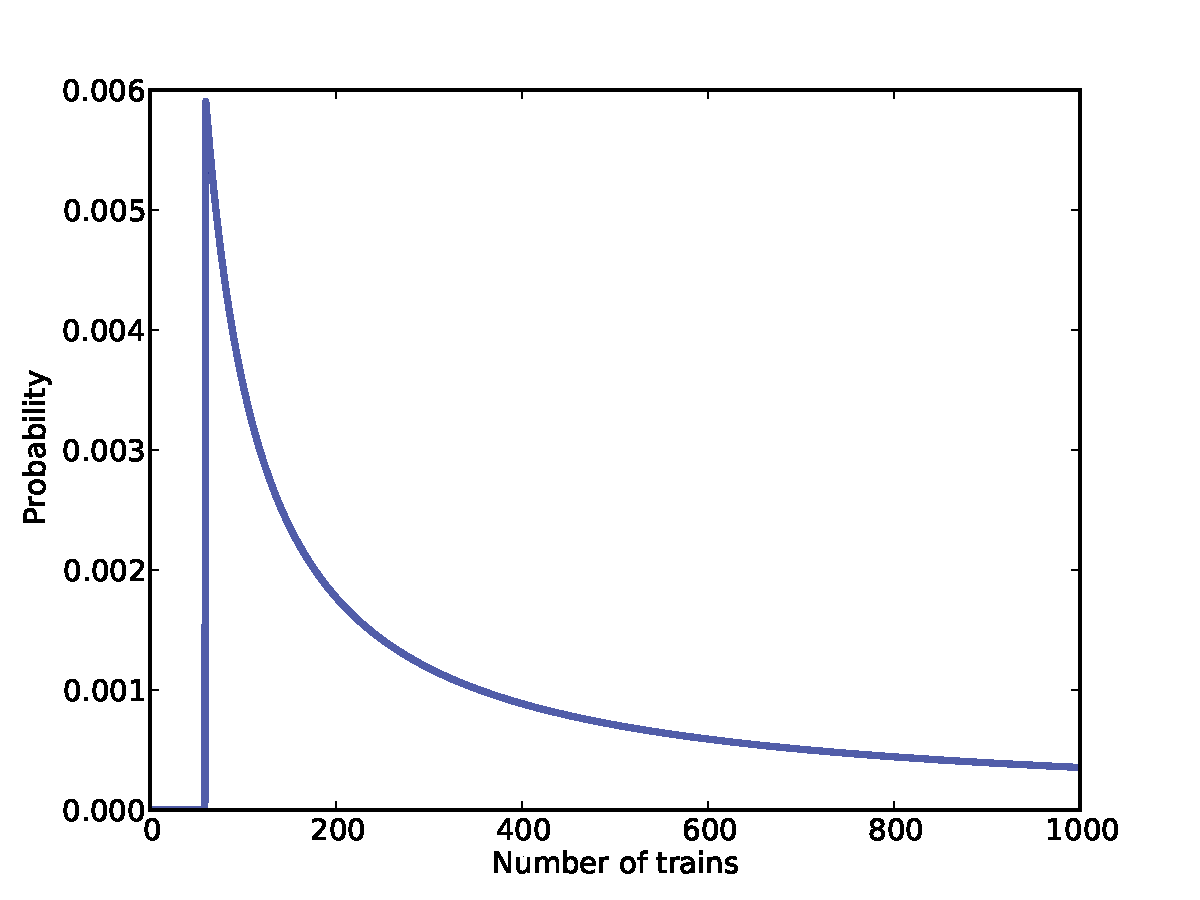
\includegraphics[height=2.5in]{figs/train1.pdf}}
\caption{Posterior distribution for the Locomotive problem, based
on a uniform prior.}
\label{fig.train1}
\end{figure}

The question doesn't give us much basis to choose a prior, but
again we can start with something simple, see what we get, and
then evaluate some alternatives.  So let's assume that $N$ is less
than 1000, and equally likely to be any value from 1 to 1000.

\begin{verbatim}
    hypos = xrange(1, 1001)
    suite = Train(hypos)
\end{verbatim}

Now all we need is a likelihood function.  With a little thought,
you will realize that the likelihood functions for the Locomotive
problem and the Dice problem are identical:

\begin{verbatim}
class Train(Suite):
    def Likelihood(self, hypo, data):
        if hypo < data:
            return 0
        else:
            return 1.0/hypo
\end{verbatim}

And here's the update:

\begin{verbatim}
    suite.Update(60)
\end{verbatim}

Since there are 1000 hypothesis, I didn't print the results.
Instead I used {\tt myplot.Pmf}:

\begin{verbatim}
    myplot.Pmf(suite)
    myplot.Show(xlabel='Number of trains',
                ylabel='Probability')
\end{verbatim}

The result is in Figure~\ref{fig.train1}.  Not surprisingly, all
values of $N$ below 60 have been eliminated.  The most likely
value, if you had to guess, is 60.  That might not seem like
a very good guess; after all, what are the chances that you just
happened to see the train with the highest number?

Nevertheless, if you want to maximize the chance of getting
the answer exactly right, you should guess 60.  But maybe that's
not the right goal.  An obvious alternative is to compute the
mean of the posterior distribution:

\begin{verbatim}
def Mean(suite):
    total = 0
    for hypo, prob in suite.Items():
        total += hypo * prob
    return total

print Mean(suite)
\end{verbatim}

Or you could use the very similar method provided by {\tt Pmf}:

\begin{verbatim}
    print suite.Mean()
\end{verbatim}

The mean of this posterior distribution is 276, so that might be a
good guess if you wanted to minimize error.  If you played this
guessing game over and over, using the mean of the posterior as your
estimate would minimize the total squared error over the long run.

You can download this example from \url{http://thinkbayes.com/train.py}.


\section{What about that prior?}

To make any progress on the Locomotive problem we had to make
some assumptions, and some of them were pretty arbitrary.  In
particular, we chose a uniform prior from 1 to 1000, without
much justification for choosing 1000, or for choosing a uniform
distribution.

It is not crazy to believe that a railroad company might operate
1000 locomotives, but a reasonable person might guess more or fewer.
So we might wonder whether the posterior distribution is sensitive
to these assumptions.  With so little data (only one observation)
it probably is.

Recall that with a uniform prior from 1 to 1000, the mean of
the posterior is 276.  With an upper bound of 500, we get a
posterior mean of 166, and with an upper bound of 2000,
the posterior mean is 467.

So that's bad.  There are two ways to proceed:

\begin{itemize}

\item Get more data.

\item Get more background information.

\end{itemize}

With more data, the posterior distributions based on different
priors tend to converge.  For example, suppose that in addition
to train 60 we also see trains 30 and 90.  We can update the
distribution like this:

\begin{verbatim}
    for data in [60, 30, 90]:
        suite.Update(data)
\end{verbatim}

With these data, the means of the posteriors are

  \begin{tabular}{|l|l|}
  \hline
  Upper & Posterior \\
  Bound & Mean \\
  \hline
  500 & 152 \\
  1000 & 164\\
  2000 & 171\\
  \hline
  \end{tabular}

So the difference between the posteriors is smaller.


\section{An alternative prior}

If more data are not available, another option is to improve the
priors by gathering more background information.  It is probably
not reasonable to assume that a railroad company with 1000 locomotives
is just as likely as a company with only 1.

With some effort, we could probably find a list of companies that
operate locomotives in the area of observation.  Or we could
interview an expert in rail shipping to gather information about
the typical size of companies.

But even without getting into the specifics of railroad economics, we
can make some educated guesses.  In most fields, there are many small
companies, fewer medium-sized companies, and only one or two very
large companies.  In fact, the distribution of company sizes tends to
follow a power law, as Robert Axtell reports in {\it Science} (see
\url{http://www.sciencemag.org/content/293/5536/1818.full.pdf}).

This law suggests that if there are 1000 companies with fewer than
10 locomotives, there might be 100 companies with 100 locomotives,
10 companies with 1000, and possibly one company with 10,000 locomotives.

Mathematically, a power law means the number of companies
with a given size is inversely proportional to the size, or
%
\[ \PMF(x) \propto \left( \frac{1}{x} \right)^{\alpha}   \]
%
where $\PMF(x)$ is the probability mass function of $x$ and $\alpha$ is
a parameter that is often near 1.

We can construct a power law prior like this:

\begin{verbatim}
class Train(Dice):
    def __init__(self, hypos, alpha=1.0):
        Pmf.__init__(self)
        for hypo in hypos:
            self.Set(hypo, hypo**(-alpha))
        self.Normalize()
\end{verbatim}

And here's the code that constructs the prior

\begin{verbatim}
    hypos = range(1, 1001)
\end{verbatim}

Again, the upper bound is arbitrary, but with a power law
prior, the posterior is less sensitive to this choice.

If we start with this prior and observe trains 30, 60 and 90,
the means of the posteriors are

  \begin{tabular}{|l|l|}
  \hline
  Upper & Posterior \\
  Bound & Mean \\
  \hline
  500 & 131 \\
  1000 & 133 \\
  2000 & 134 \\
  \hline
  \end{tabular}

Now the difference between the posteriors is much smaller.  In fact,
with an arbitrarily large upper bound, the mean converges on 134.

So the power law prior is more realistic, because it is based on
general information about the size of companies, and it
behaves better in practice.


\chapter{Urns and Coins}

\section{Four Urns}

James Joyce, the American philosopher not the Irish author, wrote
a paper called {\it How probabilities reflect evidence} that poses
the following problem (which I am quoting loosely):

\begin{quote}
Jacob and Emily both start out knowing that an urn, U, was
randomly chosen from a set of four urns ${urn_0, urn_1, urn_2, urn_3}$
where $urn_i$ contains three balls, $i$ of which are blue and $3-i$ of
which are green. [...]  Jacob and Emily regard random drawing with
replacement as an exchangeable process, so that any series of draws
that produces m blue balls and n green balls is as likely as any other
such series, irrespective of order.  Use $B^m G^n$ to denote the generic
event in which $m$ blue balls and $n$ green balls are drawn at random
and with replacement from U.  Against this backdrop of shared
evidence, suppose Jacob sees five balls drawn at random and with
replacement from U and observes that all are blue, so his evidence is
$B^5 G^0$.  Emily, who sees Jacob's evidence, looks at fifteen additional
draws of which twelve come up blue, so her evidence is $B^{17} G^3$.  [If
$B_{next}$ is the probability that the next ball drawn from the urn is
blue,] what should Emily and Jacob think about $B_{next}$?
\end{quote}

We'll proceed in two steps: the first is to compute the probability
that U is $urn_i$ for each $i$.  The second is to compute $B_{next}$.

Let's use $H_i$ to represent the hypothesis that the urn we chose, U,
is $urn_i$.  Since we are told that U was chosen at random, we can
infer that the prior probabilities are $H_i = 1/4$ for all $i$.

And the likelihood function is easy.  If $H_i$ is true, U contains
$i$ blue balls, so $\p{B|H_i} = i/3$.  Or in Python

\begin{verbatim}
class Urn(Suite):
    def Likelihood(self, hypo, data):
        """
        hypo: integer number of blue balls (out of three)
        data: string 'B' or 'G'
        """
        p = hypo / 3.0
        if data == 'B':
            return p
        else:
            return 1-p
\end{verbatim}

And here's the code that creates the prior and updates it
with Jacob's data:

\begin{verbatim}
    suite = Urn([0,1,2,3])

    for data in 'BBBBB':
        suite.Update(data)
\end{verbatim}

And here are the results:

\begin{verbatim}
0 0.0
1 0.0036231884058
2 0.115942028986
3 0.880434782609
\end{verbatim}

Since he has seen 5 blue and no green balls, Jacob rules out $urn_0$
and gives low posterior probabilities to $urn_1$ and $urn_2$.  Based
on this data, Jacob is 88\% sure that U is $urn_3$.

So what should Jacob believe about $B_{next}$, the chance that the
next ball from U is blue.  If he $H_3$ right, and U is $urn_3$,
then $B_{next}$ is 100\%.  But Jacob is not sure about $H_3$.

Jacob can compute $B_{next}$ using the law of total probability, which
says that the probability that the next ball is blue is the sum
of the probabilities for each way it can happen; in this case

\[ B_{next} = \sum i/3 \p{H_i | D} \]

Pulling out the factor of 1/3, we have

\[ B_{next} = 1/3 \sum i \p{H_i | D} \]

which we recognize as the mean of the posterior distribution, over 3.

\begin{verbatim}
print suite.Mean() / 3.0
\end{verbatim}

For Jacob, $B_{next}$ is 0.96.  For Emily, who sees 17 blue and 3 green
balls, the posterior distribution is 

\begin{verbatim}
0 0.0
1 3.05166468308e-05
2 0.999969483353
3 0.0
\end{verbatim}

Since Emily has seen a blue and a green ball, she can rule out $H_0$
and $H_3$.  And since she has seen many more blue than green balls,
she is all but certain that U is $urn_2$, so her value for $B_{next}$
is very close to 2/3.

Joyce constructed this example to point out a difference between the
evidence seen by Jacob and Emily.  Jacob's evidence has more
``force,'' in one sense of the word, because his posterior belief
about $B_{next}$ is more strongly biased.  But Emily's evidence has
more ``weight,'' because she is more confident about which urn U is.

For Joyce the point of this example is to probe what we mean
when we talk about the ``weight'' or ``force,'' of
evidence.  We will come back to this question, from a Bayesian
perspective, in the next chapter.

For us, the point of this example is to provide a warm-up exercise
that will help with the next problem.


\section{The Euro coin problem}

In {\it Information Theory, Inference, and Learning Algorithms}, David MacKay
poses this question:

\begin{quote}
A statistical statement appeared in ``The Guardian" on Friday January 4, 2002:

  \begin{quote}
        When spun on edge 250 times, a Belgian one-euro coin came
        up heads 140 times and tails 110.  `It looks very suspicious
        to me,' said Barry Blight, a statistics lecturer at the London
        School of Economics.  `If the coin were unbiased, the chance of
        getting a result as extreme as that would be less than 7\%.'
        \end{quote}

But do these data give evidence that the coin is biased rather than fair?
\end{quote}

To answer that question, we'll proceed in two steps.  The first
is to estimate the probability that the coin lands face up.  The second
is to evaluate whether the data support the hypothesis that the
coin is biased.

Any given coin has some probability, $x$, of landing heads up when spun
on edge.  It seems reasonable to believe that the value of $x$ depends
on some physical characteristics of the coin, primarily the distribution
of weight.



\begin{verbatim}
\end{verbatim}

\begin{verbatim}
\end{verbatim}

\begin{verbatim}
\end{verbatim}

\begin{verbatim}
\end{verbatim}

\begin{verbatim}
\end{verbatim}

\begin{verbatim}
\end{verbatim}


\end{document}
